% REMEMBER: Write the thesis from the view of the reader. How would I like to READ the thesis?
% WHY -> WHAT -> HOW structure

\chapter{Testing With Whisker}

\mnote{TODO: explain how tests are run $\rightarrow$ any Scratch VM, Whisker has a GUI for it, TAP13 reports}
\mnote{TODO: explain automated test input generation}
\mnote{TODO: explain why the program is loaded before each test}
% - Before starting a test case, the project is loaded to make sure that every test starts with the same program state
%     - If this would not be done, it would be very hard to test programs that don't do proper initialization
%     - Tests would depend on the state the previous test leaves the program in, since Scratch programs don't reset when being stopped
%     $\rightarrow$ Very inconsistent, therefore desirable to load the program before each test

\section{General Approach}

In this work, we propose a way to perform dynamic testing on Scratch programs.
The main goal of this approach is to be able to automatically assess student's solutions to Scratch assignments.
In order to do so, this approach makes use of an automation utility, which allows test code to interact with a running Scratch program.
% To enable dynamic testing for Scratch, we propose a black-bock approach with a testing utility, which allows test code to interact with a running Scratch program.
\parspace

Because Scratch's parallel scripts, as well as its lack of code separation, would make white-box testing difficult,
we instead chose to ignore the internals of the program and to go with a black-box approach, which only focuses on the program's input and output.
This raises the question of how to access Scratch's IO.
Since Scratch's input usually consists of mouse and keyboard input, and its output consists of visual animations and sound,
they are not easily accessible in a programmable way.
To overcome this challenge, we developed an automation utility called Whisker, which acts as a wrapper around Scratch.
It interacts with Scratch's virtual machine in order to automate its IO.
Whisker offers a programmable interface for Scratch, which makes automated testing for Scratch possible.
\mnote{TODO: reference figure in the text}
\parspace

Whisker is, like Scratch 3.0, implemented in JavaScript.
Hence, test code is also written in JavaScript.
Whisker can, in theory, be used with any JS testing framework,
but for compatibility reasons, we developed a rudimentary testing framework to go along with Whisker (more on this in section~\ref{TODO}).


% Therefore, we only concern ourselves with ...

% We are going to deal with this problem by creating a wrapper around Scratch,
% which can be used to simulate input and access information about the sprites which make up the output.
% Tests can then use methods, which the wrapper provides, instead of manually interacting with the Scratch program.

% Therefore, additional computations by the testing procedure must be fast enough to avoid interfering with the program under test.

\mnote{TODO: better captions for figures}
\begin{figure}[ht]
    \centering

    \begin{subfigure}[b]{\textwidth}
        \centering
        \tikzset{>=latex,
               arrow/.style={draw, -{Latex[length=1.5mm, width=1.5mm]}},
                 put/.style={draw, minimum height=1.7cm, minimum width=3.5cm, rounded corners, fill=red!20, text width=2.5cm, text centered},
                  vm/.style={draw, minimum height=3.0cm, minimum width=6.0cm, rounded corners, fill=white},
                 gui/.style={draw, minimum height=4.2cm, minimum width=7.0cm, rounded corners, fill=blue!20},
                 box/.style={draw, minimum height=4.2cm, minimum width=4.0cm, rounded corners, text width=3.5cm},
              boxtxt/.style={minimum width=4.0cm, rounded corners, text width=3.5cm}}

         \begin{tikzpicture}[scale=0.8, every node/.style={scale=0.8}]
            \begin{scope}[on background layer]
                \node[gui] at (0.0,  0.4) (gui)     {};
                \node[vm]  at (0.0,  0.0) (vm)      {};
            \end{scope}

            \node[put]     at (0.0, -0.4) (put)     {\textbf{Program under test}};
            \node[]        at (0.0,  1.0) (vmtxt)   {\textbf{Scratch Virtual Machine}};
            \node[]        at (0.0,  2.0) (guitxt)  {\large \textbf{Scratch GUI}};
            \node[box, left=of gui]       (input)   {};
            \node[box, right=of gui]      (output)  {};
            \node[boxtxt, below right] at ([yshift=-2mm] input.north west)  (inputtxt)
                {\centering {\large \textbf{Input}}\\[.5\baselineskip]Key presses, mouse movement, mouse clicks, etc.};
            \node[boxtxt, below right] at ([yshift=-2mm] output.north west) (outputtxt)
                {\centering {\large \textbf{Output}}\\[.5\baselineskip]Visual animations, audio, etc.};

            \path [arrow] (input) -- (gui);
            \path [arrow] (gui)   -- (output);
        \end{tikzpicture}
        \caption{Input and output of the Scratch GUI}
        \label{fig:input_and_output_of_the_scratch_gui}
    \end{subfigure}

    \bigskip

    \begin{subfigure}[b]{\textwidth}
        \centering
        \tikzset{>=latex,
               arrow/.style={draw, -{Latex[length=1.5mm, width=1.5mm]}},
                 put/.style={draw, minimum height=1.7cm, minimum width=3.5cm, rounded corners, fill=red!20, text width=2.5cm, text centered},
                  vm/.style={draw, minimum height=3.0cm, minimum width=6.0cm, rounded corners, fill=white},
             whisker/.style={draw, minimum height=4.2cm, minimum width=7.0cm, rounded corners, fill=green!20},
                 box/.style={draw, minimum height=4.2cm, minimum width=4.0cm, rounded corners, text width=3.5cm},
              boxtxt/.style={minimum width=4.0cm, rounded corners, text width=3.5cm}}

         \begin{tikzpicture}[scale=0.8, every node/.style={scale=0.8}]
            \begin{scope}[on background layer]
                \node[whisker] at (0.0,  0.4) (whisker) {};
                \node[vm]      at (0.0,  0.0) (vm)      {};
            \end{scope}

            \node[put]         at (0.0, -0.4) (put)     {\textbf{Program under test}};
            \node[]            at (0.0,  1.0) (vmtxt)   {\textbf{Scratch Virtual Machine}};
            \node[]            at (0.0,  2.0) (guitxt)  {\large \textbf{Scratch GUI}};
            \node[box, left=of whisker]       (input)   {};
            \node[box, right=of whisker]      (output)  {};
            \node[boxtxt, below right] at ([yshift=-2mm] input.north west)  (inputtxt)
                {\centering {\large \textbf{Input}}\\[.5\baselineskip]Calls to input simulating interface methods};
            \node[boxtxt, below right] at ([yshift=-2mm] output.north west) (outputtxt)
                {\centering {\large \textbf{Output}}\\[.5\baselineskip]Interface to query information about sprites and variables};

            \path [arrow] (input)   -- (whisker);
            \path [arrow] (whisker) -- (output);
        \end{tikzpicture}
        \caption{Input and output of Whisker}
        \label{fig:input_and_output_of_whisker}
    \end{subfigure}

    \caption{Comparison of IO mechanisms}
    \label{fig:comparison_of_io_mechanisms}
\end{figure}

\section{Public Interface}

\mnote{TODO: better explanations and code examples}
Automating Scratch allows us to write tests for Scratch in a unit-test-like fashion.
Whisker loads and starts the program before each test starts.
By doing this, every test starts with a fresh instance of the program in the exact same situation.
The test code can then interact with the program in order to produce a desired situation and check how the program behaves through assertions.
\parspace

\mnote{TODO: properties depend on time $\rightarrow$ ''old'' values}
The following list will give an overview of Whisker's basic functions.
The Whisker instance will be denoted as $t$ in example code snippets.

\begin{itemize}
    \item \textbf{Simulate Input.}
        \mnote{TODO: check if key is pressed}
        By simulating Scratch's main input methods, the test can control the tested program.
        The goal is to simulate a user interacting with the program.
        Therefore, this is the only way the test can manipulate the program.
        The possible input includes mouse movement, mouse button presses, keyboard key presses and entering answers to ask blocks.
        \begin{javascriptcode}
            t.addInput(1000, {
                device: 'keyboard',
                key: 'right arrow',
                isDown: true
            });
        \end{javascriptcode}
    \item \textbf{Access Information.}
        \mnote{Explain how in the implementation chapter (objects)}
        The testing utility can be used to access sprites and variables of the program.
        This makes it possible to gather information about anything, which is displayed on the stage.
        Analyzing Scratch's visual output would otherwise be very difficult.
        The provided sprite attributes include the sprite's position, rotation, size, current costume, speech bubble text, etc..
        The values of the program's variables can also be accessed.
        These variable values can usually be displayed to the user in Scratch's graphical output, and are commonly used in Scratch programs to convey information to the user.
        \begin{javascriptcode}
            const sprite = t.getSprite('Sprite1');
            const stage = t.getStage();
            const variable = stage.getVariable('my variable');
            console.log(sprite.x);
            console.log(variable.value);
        \end{javascriptcode}
    \item \textbf{Control the program execution.}
        The test is able to control when and for how long the program under test is run.
        In the beginning of the test, the program starts in a paused state with the green flag already pressed.
        The test can then run (resume) the program for a certain time, or until a condition is met.
        The green flag can also be pressed again in order to restart the program, which can, for example, be useful for testing programs, that use randomness.
        \begin{javascriptcode}
            await t.runForTime(1000);
            await t.runUntil(() => sprite.x > 100));
            t.greenFlag();
        \end{javascriptcode}
    \item \textbf{Register Callbacks.}
        The test can register callbacks, which get called every time Scratch renders a new picture.
        This allows the test to track the information, which the user would normally see, while the program is running.
        \begin{javascriptcode}
            const spritePositions = [];
            const callback = t.addCallback(() => spritePositions.push(sprite.pos));
            callback.disable();
            callback.enable();
        \end{javascriptcode}
    \item \textbf{Register constraints.}
        By registering constraints, the test can define conditions that must always hold true.
        Constraints are done through special callbacks, which perform assertions.
        For example, this can be used to define that a certain sprite must always be visible.
        \begin{javascriptcode}
            const constraint = t.addConstraint(() => {
                t.assert.ok(sprite.visible === true)
            });
            constraint.disable();
            constraint.enable();
        \end{javascriptcode}
\end{itemize}

\noindent Despite being possible in theory, Whisker does not provide the means to execute single scripts or blocks of the program directly.
\mnote{TODO: really write about grading here?}
It only allows executing the program as a whole.
This has two reasons.
Since the main goal for this testing approach is automated grading, one test suite is possibly executed on a large number of different implementations.
Therefore, we don't want to concern ourselves with the internals of the program, since they may change from program to program.
Secondly, executing single scripts could also lead to unexpected behaviour in the program, because scripts in typical Scratch programs often depend on other scripts, which run in parallel.
% This is mainly due to the game-like nature of usual Scratch programs.
% They often feature multiple sprites running loops in order to be interactive.

\section{Advantages and Disadvantages}

\mnote{TODO: better explanations, better intro, small discussion}
This section will highlight some advantages and disadvantages of the presented testing approach.
\parspace

% - Scratch programs can be pretty inconsistent
%     - Some programs may only sometimes work and other times not
%     $\rightarrow$ They may or may not pass the test

\noindent Disadvantages:

\begin{itemize}
    \item Scratch programs have to be well specified, since testing relies on the program's specification.
        Therefore, if the specification is too vague, testing can become difficult.
        Tests for imprecise specifications potentially need to consider more possible cases of how the program could behave.
        Likewise, conflicting interpretations of the specification between the test and the program may result in false negative test outcomes.
    \item Since we only test the program as a whole, testing a single part of the program can be difficult.
        If, for example, some functionality of a program depends on another functionality being implemented correctly,
        but the latter does not work, we can not test the first functionality properly.
\end{itemize}

\noindent Advantages:

\begin{itemize}
    \item This approach allows to test programs with most of Scratch's functionality.
        Apart from sounds and extensions, anything, which Scratch has to offer, can be tested with this approach.
        In contrast, ITCH's previous testing approach limited Scratch programs to textual IO.
    \item Tests are easily understood, because they control the program like a normal person would.
    \mnote{Can't state this without proof $\rightarrow$ just say that test use the program like a normal person $\rightarrow$ e.g. recorded input could be used}
        This is important, because students, whose programs are supposed to be tested later,
        could be allowed to run tests on their programs themselves during development.
        This way, students could easily receive valuable feedback about the correctness of their implementations.
        Therefore, it is beneficial to use tests, whose actions and purposes are easily understood by students.
\end{itemize}

\section{Challenges of this Approach}

% \textbf{Absolute timings.}
% Scratch offers code blocks to delay the execution of a script, which often find use in typical game-like programs.
% These blocks use absolute timings to implement the delay.
% Basically, they save the current time when they pause the script,
% then later resume the execution of the script when the difference between the current time and the saved time reached the desired delay length.
% This means, that the execution of the Scratch program can only be paused or delayed for a very short time without interfering with these timings.
% Pausing the execution of the Scratch program for too long, while a delay is active,
% takes away execution time from other scripts, which are executed parallel to the delay.
% This can potentially have an impact on the program under test.
% % Therefore, additional computations by the testing procedure must be fast enough to avoid interfering with the program under test.
% \mnote{TODO: Reference the evaluation section about timings here?}
% \mnote{TODO: Rewrite this with an example so it's easier to understand}
%
% \begin{figure}[ht]
%     \centering
%     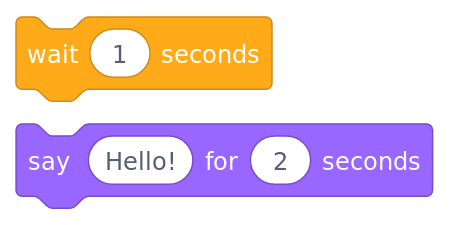
\includegraphics[width=0.30\textwidth]{code-timing}
%     \caption{Delaying blocks}
%     \label{fig:delaying_blocks}
% \end{figure}
%
% TODO: actions don't necessarily happen in the same step -> have to track timings

\chapter{Using Constraints For Flexible Test Inputs}%
\label{cha:using_constraints_to_enable_flexible_test_inputs}

This section will describe why separating control of the program under test from the test code can be beneficial,
and how this can be achieved by using Whisker's  mechanism to define constraints.

\section{Input-Independent Tests}

Usually, tests will provide the program under test with inputs and check the resulting outputs.
However, in many cases, a different approach is possible as well.
Tests may use other sources of input and simply observe if the program's output is correct for the input provided by the source.
QuickCheck~\cite{quickcheck} by Claessen et al., for example, uses this principle, to test the correctness of Haskell programs.
In order to do so, tests define conditions, which the program must comply with.
QuickCheck then automatically generates input for the program and checks if the defined conditions hold.
\parspace

Scratch programs can often be tested in a similar way.
But in order to be able to do this, tests have to be made independent of the simulated input on the program.
This will not just enable us to test with random input, but with other input sources as well.
For example, the program could be manually controlled by a person, or input could be recorded and played back.
Whisker also offers its own method of automated input generation by randomizing a set of inputs,
which are either provided by the test itself, or deduced by analyzing the program code (see section~\ref{TODO} for more information on this).
\parspace

Scratch tests can be made independent of inputs, and Whisker provides the means to do this.
Using constraints allows us to define conditions, which the program must hold.
Constraints check the programs compliance to the conditions by continually performing assertions throughout the program execution.
Since this is done entirely in the background while the program under test is running, we can define some constraints and just let the program run for some time.
This way, it does not matter in what state the program is during its execution, or what inputs it is receiving.
If a condition does not hold, the respective constraint fails.

\section{Input-Independent Testing Procedure}

Figure~\ref{fig:input-independent-testing-procedure} shows a testing procedure, which uses the aforementioned approach to test independently of the simulated input.
We will go through each step of the procedure with the aid of an example.
Consider a program with a single sprite, which is supposed to move to the right precisely when the right arrow key is pressed.
We want to write a test to check if the sprite's movement works correctly.

\begin{figure}[ht]
    \centering
    \tikzset{>=latex,
           arrow/.style={draw, -{Latex[length=1.5mm, width=1.5mm]}},
             box/.style={draw, text width=4.3cm, minimum height=0.7cm, text centered, rounded corners},
             num/.style={draw, circle, inner sep=0.6mm, text centered},
               h/.style={fill=blue!10}}

     \begin{tikzpicture}[scale=0.9, every node/.style={scale=0.9}]
        \node[box, h] at ( 0.2,  4.25) (tracking)    {Setup information tracking};
        \node[box, h] at ( 0.2,  3.0)  (constraints) {Register constraints};
        \node[box]    at ( 0.2,  2.0)  (inputs)      {(Simulate Inputs)};
        \node[box]    at ( 0.2,  1.0)  (run)         {Run the program};
        \node[box, h] at ( 0.2,  0.0)  (verify)      {Verify tested situation};

        \node[num] at (-2.6,  4.25) (one)   {1};
        \node[num] at (-2.6,  3.0)  (two)   {2};
        \node[num] at (-2.6,  2.0)  (three) {3};
        \node[num] at (-2.6,  1.0)  (four)  {4};
        \node[num] at (-2.6,  0.0)  (five)  {5};

        \draw[arrow]
               ( 0.2,  5.1)
            -- (tracking)
            -- (constraints)
            -- (inputs)
            -- (run)
            -- (verify)
            -- ( 0.2, -0.8);
    \end{tikzpicture}
    \caption{Input-Independent Testing Procedure}
    \label{fig:input-independent-testing-procedure}
\end{figure}

\begin{enumerate}
    \item \textbf{Setup information tracking.}
        \mnote{TODO: Update for new example}
        The constraint, which we will have to define later, will depend on information, which is not always available.
        Because we need to determine the sprite's movement direction, we have to know the position of the sprite from the last rendered frame.
        In order to track this, we add a callback, which tracks the sprite's last position.
        (Note: Whisker makes the sprites' attributes from the last rendered frame available through \texttt{sprite.old}, but we are going to ignore this for the sake of the example)
        \begin{javascriptcode}
            let oldX;
            t.addCallback(() => {
                oldX = sprite.x;
            });
        \end{javascriptcode}
    \item \textbf{Register constraints.}
        Now, that we know the sprite's last position, we can determine if, and in which direction, it has moved since the last frame.
        We check its movement dependent on what key is currently pressed.
        \begin{javascriptcode}
            t.addConstraint(() => {
                if (t.isKeyDown("right arrow")) {
                    t.assert.ok(sprite.x > oldX);
                } else {
                    t.assert.ok(sprite.x === oldX);
                }
            });
        \end{javascriptcode}
    \item[3+4.] \textbf{Simulate Inputs, Run the program.}
        \setcounter{enumi}{4}
        Now we can register inputs if we want to, and then we can run the program.
        How we simulate inputs, or if we perform inputs manually, does not matter for the test, of course.
        \begin{javascriptcode}
            t.detectRandomInputs();
            await t.runForTime(5000);
        \end{javascriptcode}
    \item \textbf{Verify tested situation.}
        If our source of input does not guarantee, that the right arrow key gets pressed at all, we risk the chance of a false positive test result,
        because then, part of our constraint does not ever get checked.
        In this case, we also want set up tracking for the key press in the beginning,
        and then skip the test if the key does not get pressed at all in the end.
        \begin{javascriptcode}
            let rightPressed = false;
            const detectRight = t.addCallback(() => {
                if (t.isKeyDown("right arrow")) {
                    rightPressed = true;
                    detectRight.disable();
                }
            });

            ...

            t.assume.ok(rightPressed);
        \end{javascriptcode}
\end{enumerate}

\begin{listing}[ht]
    \centering
    \begin{subfigure}[b]{.35\textwidth}
        \centering
        \begin{minted}[autogobble, breaklines, linenos, fontsize=\tiny, framesep=2mm, frame=lines]{javascript}
            const sp = t.getSprite('Sprite1');

            let oldX = sprite.x;

            await t.runForTime(1000);

            /* Sprite should not move when no key
               is pressed. */
            t.assert.ok(oldX === sprite.x);

            t.inputImmediate({
                device: 'keyboard',
                key: 'right arrow',
                isDown: true
            });

            await t.runForTime(1000);

            /* Sprite should move right when the
               right arrow key is pressed. */
            t.assert.ok(oldX < sprite.x);
        \end{minted}
        \caption{Normal test}
    \end{subfigure}
    \hspace{.08\textwidth}
    \begin{subfigure}[b]{.55\textwidth}
        \centering
        \mnote{TODO: update comments}
        \begin{minted}[autogobble, breaklines, linenos, fontsize=\tiny, framesep=2mm, frame=lines]{javascript}
            const sprite = t.getSprite('Sprite1');

            /* Give the program some time to initialize itself. */
            await t.runForTime(100);

            /* (1) Track when the right arrow key is being pressed,
             * and when it is released. */
            let startPressedTime,  pressedTime;
            let startReleasedTime, releasedTime;
            let currentlyPressed = t.isKeyDown('right arrow');
            t.addCallback(() => {
                const currentTime = t.getTotalTimeElapsed();
                if (t.isKeyDown('right arrow')) {
                    pressedTime = currentTime;
                    if (!currentlyPressed) {
                        startPressedTime = currentTime;
                        currentlyPressed = true;
                    }
                } else {
                    releasedTime = currentTime;
                    if (currentlyPressed) {
                        startReleasedTime = currentTime;
                        currentlyPressed = false;
                    }
                }
            });

            /* (1) Track when the sprite is moving to the right,
             * and when it is staying still. */
            let movedRightTime;
            let stayedStillTime;
            t.addCallback(() => {
                if (sprite.x > sprite.old.x) {
                    movedRightTime = t.getTotalTimeElapsed();
                } else if (sprite.x === sprite.old.x) {
                    stayedStillTime = t.getTotalTimeElapsed();
                }
            });

            /* (2) Check if the sprite only moves when the right arrow
             * key was pressed, and if it doesn't move when the key was
             * not pressed. */
            t.addConstraint(() => {
                const currentTime = t.getTotalTimeElapsed();
                if (currentTime > startPressedTime + 100) {
                    t.assert.ok(pressedTime - movedRightTime <= 100,
                                'Sprite must move right when right arrow key is pressed.');
                }
                if (currentTime > startReleasedTime + 100) {
                    t.assert.ok(releasedTime - stayedStillTime <= 100,
                                'Sprite must not move right when right arrow key is not pressed.');
                }
            });

            /* (3) Some code, which registers inputs. Or nothing if
             * inputs are done manually. For example, generated input: */
            t.setRandomInputInterval(250);
            t.detectRandomInputs();

            /* (4) Run the program. */
            await t.runForTime(5000);

            /* (5) Check if the right arrow key was pressed at all,
             * and if it was ever released. */
            t.assume.ok(pressedTime > 0, 'Right arrow key must be pressed.');
            t.assume.ok(releasedTime > 0, 'Right arrow key must be released.');
        \end{minted}
        % \begin{minted}[autogobble, breaklines, linenos, fontsize=\scriptsize, framesep=2mm, frame=lines]{javascript}
        %     const sprite = t.getSprite('Sprite1');
        %
        %     /* Detect if the right key is pressed.
        %        Optional, if  the used input guarantees,
        %        that the right arrow key is pressed. */
        %     let rightPressed = false;
        %     const detectRight = t.addCallback(() => {
        %         if (t.isKeyDown("right arrow")) {
        %             rightPressed = true;
        %             detectRight.disable();
        %         }
        %     });
        %
        %     /* (1) Track the x position of the sprite, so
        %        horizantal movement can be checked. */
        %     let oldX;
        %     t.addCallback(() => {
        %         oldX = sprite.x;
        %     });
        %
        %     /* (2) Sprite should move right when the
        %        right arrow key is pressed. Sprite
        %        should not move when no key is pressed. */
        %     t.addConstraint(() => {
        %         if (t.isKeyDown("right arrow")) {
        %             t.assert.ok(sprite.x > oldX);
        %         } else {
        %             t.assert.ok(sprite.x === oldX);
        %         }
        %     });
        %
        %     /* (3) Some code, which registers inputs.
        %        Or nothing if inputs are done manually.
        %        For example: */
        %     t.detectRandomInputs();
        %
        %     /* (4) */
        %     await t.runForTime(5000);
        %
        %     /* (5) Optional, if  the used input
        %        guarantees, that the right arrow key
        %        is pressed. */
        %     t.assume.ok(rightPressed);
        % \end{minted}
        \caption{Input-independent test}
    \end{subfigure}
    \caption{Comparison of normal tests and an input-independent tests}
    \label{fig:normal-input-independent-test-comparison}
\end{listing}
\parspace

Figure~\ref{fig:normal-input-independent-test-comparison} shows the resulting test code for the example
and compares it to a similar test, which simulates inputs deliberately to check the sprite's movement.
We can easily see, that this approach is quite a bit more costly than the more normal approach.
But at the same time, the input-independent testing procedure is able to scale better than the other testing procedure.
Once enough tracking is set up, writing constraints becomes easy and does not requires little code.
At the same time, because the constraints are isolated from the program execution itself,
many constraints can possibly be combined into a single test.
For this purpose, Whisker offers an option to disable failed constraints instead of failing the entire test.
Hence, the test can simply check which constraints failed at the end, and let Whisker generate a test report from them.

% Apart from being independent of their test input, a second advantage of this approach is that it allows tests to easily be combined.
% By copying constraints and their necessary tracking from one test to another, the checks of one test can be combined with the other's checks.
% Depending on the program, it may be possible to perform many tests with a single program execution.
% In case tests are expected to fail, Whisker also offers the option to simply disable failed constraints instead of failing the test.
% This way, the test can simply check which constraints failed at the end, and let Whisker generate a test report from them.

\mnote{TODO: figure}

% \begin{figure}[ht]
%     \centering
%     \begin{subfigure}[b]{.45\textwidth}
%         \centering
%         \tikzset{>=latex,
%                  box/.style={draw, text width=4.3cm, minimum height=0.7cm, text centered, rounded corners},
%                  num/.style={draw, circle, inner sep=0.6mm, text centered},
%                    h/.style={fill=blue!10}}
%
%         \begin{tikzpicture}
%             \node[box] at ( 0.2,  3.0) (run)        {Run the program};
%             \node[box] at ( 0.2,  2.0) (inputs)     {Simulate inputs};
%             \node[box] at ( 0.2,  1.0) (checks)     {Perform checks};
%
%             \node[num] at (-2.6,  3.0) (one)   {1};
%             \node[num] at (-2.6,  2.0) (two)   {2};
%             \node[num] at (-2.6,  1.0) (three) {3};
%
%             \draw[->]
%                    ( 0.2,  4.8)
%                 -- (run)
%                 -- (inputs)
%                 -- (checks)
%                 -- ( 0.2, -1.0);
%
%             \draw[shorten >= 2pt, rounded corners, dashed, ->]
%                    ( 0.2,  0.0)
%                 -- (-3.4,  0.0)
%                 -- (-3.4,  4.0)
%                 -- ( 0.2,  4.0);
%         \end{tikzpicture}
%
%         \caption{Normal Test Procedure}
%         \label{fig:normal_test_procedure}
%     \end{subfigure}
%     \begin{subfigure}[b]{.45\textwidth}
%         \centering
%         \tikzset{>=latex,
%                  box/.style={draw, text width=4.3cm, minimum height=0.7cm, text centered, rounded corners},
%                  num/.style={draw, circle, inner sep=0.6mm, text centered},
%                    h/.style={fill=blue!10}}
%
%         \begin{tikzpicture}
%             \node[box] at ( 0.2,  4.25) (tracking)    {Setup tracking of information};
%             \node[box] at ( 0.2,  3.0)  (constraints) {Register constraints};
%             \node[box] at ( 0.2,  2.0)  (run)         {Run the program};
%             \node[box] at ( 0.2,  1.0)  (inputs)      {(Simulate Inputs)};
%             \node[box] at ( 0.2,  0.0)  (filter)      {Filter constraints};
%
%             \node[num] at (-2.6,  4.25) (one)   {1};
%             \node[num] at (-2.6,  3.0)  (two)   {2};
%             \node[num] at (-2.6,  2.0)  (three) {3};
%             \node[num] at (-2.6,  1.0)  (four)  {4};
%             \node[num] at (-2.6,  0.0)  (five)  {5};
%
%             \draw[->]
%                    (tracking)
%                 -- (constraints)
%                 -- (run)
%                 -- (inputs)
%                 -- (filter)
%                 -- ( 0.2, -1.0);
%         \end{tikzpicture}
%
%         \caption{Constraint-only Test Procedure}
%         \label{fig:constraint_only_test_procedure}
%     \end{subfigure}
%     \caption{Comparison of the procedure of normal tests and constraint-only tests}
%     \label{fig:comparison_of_the_procedure_of_normal_tests_and_constraint_only_tests}
% \end{figure}
